\chapter{Regression Tests}
Figure \ref{ACLTEST} shows the layout of the test suites in the ACL. To run the complete test, we need only run the file \texttt{Test\_Tests}. Since the total test may last a few minutes, the tests are additionally divided into five main categories: \texttt{Test-Big\_Number}, \texttt{Test-Symmetric\_Ciphers}, \texttt{Test-Asymmetric\_Ciphers}, \texttt{Test-Hash} and \texttt{Test-MISC}. All test cases for the big number library are in \texttt{test\_suite\_big\_num1}, \texttt{test\_suite\_\-big\_num2}, \texttt{test\_suite\_big\_num3} and \texttt{test\_suite\_big\_num4}, the four suites are then collected in \texttt{test\_suite\_big\_num\_all}.
\begin{figure}[h]
  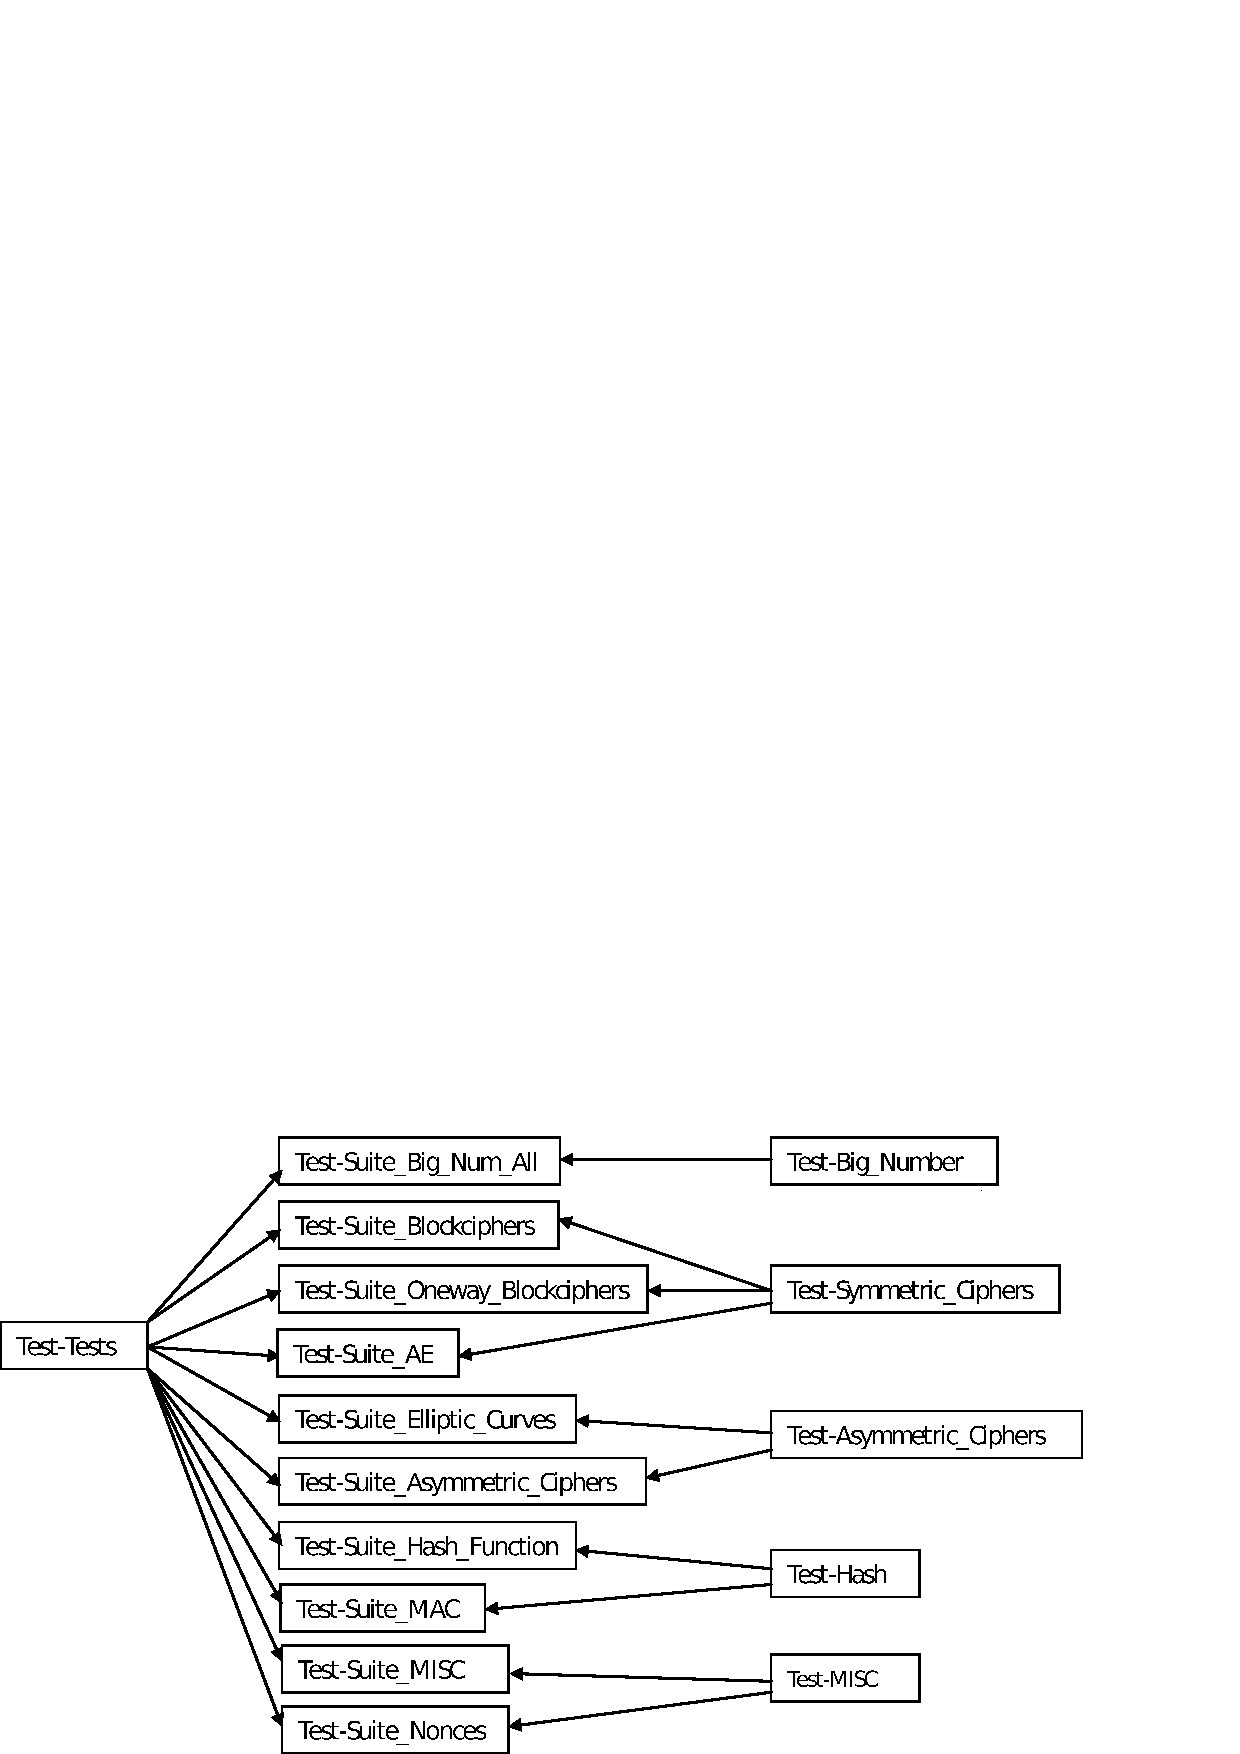
\includegraphics[scale=0.8]{Pictures/Layout_of_Test_Suite.pdf} 
  \caption{The structure of the ACL Test.}\label{ACLTEST}
\end{figure}

We start by writing a simple test case for the package \texttt{Crypto.Types.Big\_Numbers}.
\begin{lstlisting}[numbers=left,caption={test-big\_number\_power.ads}\label{Big12}]
 with AUnit;
 with AUnit.Test_Cases;
 with Ada.Strings.Unbounded;  
 package Test.Big_Number_Power is
   use AUnit;
   use Ada.Strings.Unbounded;
   type Big_Number_Test is new Test_Cases.Test_Case with null record;
 
   procedure Register_Tests(T: in out Big_Number_Test);
   function Name(T: Big_Number_Test) return Test_String;
   procedure Big_Number_Test1(T: in out Test_Cases.Test_Case'Class);
 end Test.Big_Number_Power;
\end{lstlisting}

\begin{lstlisting}[numbers=left,caption={test-big\_number\_power.adb}\label{Big1}]
 with AUnit.Assertions; 
 with Crypto.Types.Big_Numbers;
 pragma Elaborate_All(Crypto.Types.Big_Numbers);
 package body Test.Big_Number_Power is
  package Big is new Crypto.Types.Big_Numbers(512);
  use Big;
  use Big.Utils;
  A: Big_Unsigned := To_Big_Unsigned("19");
  Result:Big_Unsigned:= To_Big_Unsigned("1978419655660313589123979");
	
  procedure Register_Tests(T : in out Big_Number_Test) is
	use Test_Cases.Registration;
  begin
	Register_Routine(T, Big_Number_Test1'Access,"Power");
  end Register_Tests;

  function Name(T : Big_Number_Test) return Test_String is
  begin
	return new String'("Big Number Tests");
  end Name;

  procedure Big_Number_Test1(T: in out Test_Cases.Test_Case'Class) is
    use AUnit.Assertions; 
  begin
    Assert(A ** A = Result, "Failed with A.");
  end Big_Number_Test1;
 end Test.Big_Number_Power;
\end{lstlisting}

Listing \ref{Big12} is the header file, which contains the definitions of the types and operations required for the corresponding body file. As shown in Listing \ref{Big1}, the function \texttt{Register\_Tests()} (line 12) registsters the test case \texttt{Big\_Number\_Test1}, and the function \texttt{Name()} (line 18) returns the name of the test case. The procedure \texttt{Big\_Number\_Test1()} (line 23) contains the test case, which tests if $19^{19}$ equals the result or not. The method \texttt{Assert()} (line 26) checks the values, if the two values are equal, then, the test is passed, else, the test case is failed with a message "Failed with A." printed. 

\begin{lstlisting}[numbers=left,caption={test-suite\_big\_number.ads}\label{BigS2}]
 with AUnit; use AUnit;
 with AUnit.Test_Suites;
 package Test.Suite_Big_Num is
   function Suite return Test_Suites.Access_Test_Suite;
 end Test.Suite_Big_Num;
\end{lstlisting}

\begin{lstlisting}[numbers=left,caption={test-suite\_big\_number.adb}\label{BigS}]
 with Test.Big_Number_Power;
 package body Test.Suite_Big_Num is
  Result	    : aliased Test_Suite;
  Test_Power : aliased Test.Big_Number_Power.Big_Number_Test;  
  function Suite return Access_Test_Suite is
  begin
    Add_Test(Result'Access, Test_Power'Access);    
    return Result'Access;
  end Suite;
 end Test.Suite_Big_Num;
\end{lstlisting}

Figure \ref{BigS2} is the header file of a test suite, and
Figure \ref{BigS} is the body file. As shown in Figure \ref{BigS}, the function \texttt{Suite()} (line 5) gathers the test cases from the file \texttt{Test.Big\_Number\_Power}.

\begin{lstlisting}[numbers=left,caption={test-big\_number.adb}\label{BigR}]
 with Test.Suite_Big_Num;
 with AUnit.Run;
 with AUnit.Reporter.Text;
 procedure Test.Big_Number is
   procedure Run is new AUnit.Run.Test_Runner_With_Results
   							(Test.Suite_Big_Num.Suite);
   Reporter : AUnit.Reporter.Text.Text_Reporter;
 begin
   Run(Reporter); 
 end Test.Big_Number;
\end{lstlisting}

To run the tests, a runner (Figure \ref{BigR}) is created to provide a routine that execute all the test cases in the suite. Test results are reported using \texttt{Reporter}, which is specified when calling \texttt{Run}. The final report is output once all test have been run, so that they can be grouped (failed or passed).
We need only compile the file \texttt{test-big\_Number.adb}.
Figure \ref{TEST} shows the test result for the package \texttt{Crypto.Types.Big\_Numbers}.
\begin{figure}[h]
\centering
  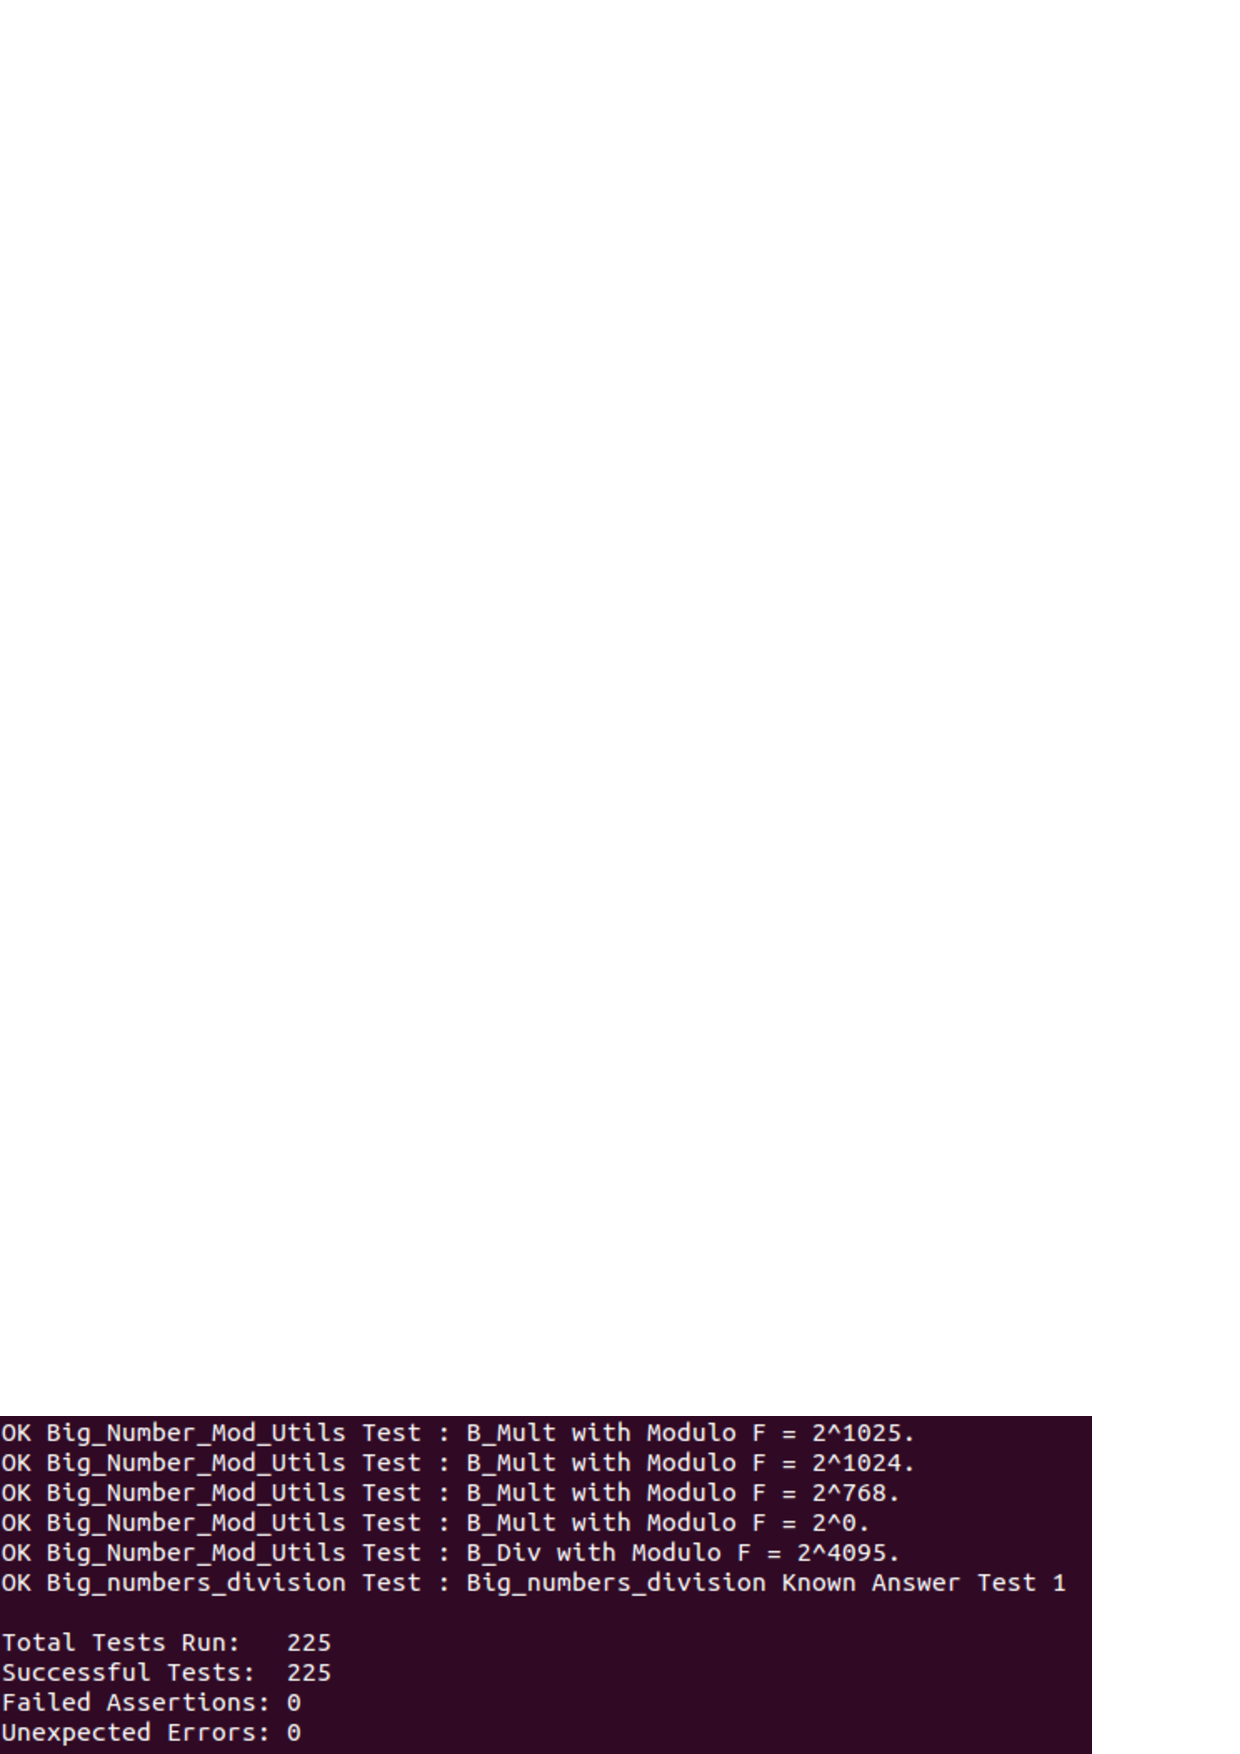
\includegraphics[scale=0.5]{Pictures/Big_Number.png} 
  \caption{The result of a test.}\label{TEST}
\end{figure}

This is the same workflow when we do other tests. To run the whole test cases, we need to compile the file \texttt{test-tests.adb}, it is the runner, which collects all test suites for the ACL.